\documentclass[aspectratio=169]{beamer}

\mode<presentation> {
\usetheme{default}
\setbeamertemplate{footline}[page number]
\setbeamertemplate{navigation symbols}{}
\setbeamertemplate{caption}{\raggedright\insertcaption\par}
}

\usepackage{graphicx}
\usepackage{booktabs}
\usepackage{amsmath}
\usepackage{listings}
\usepackage{multicol}
\usepackage{pdfpcnotes}

\title[Autocorrelation Wavelets]{Data Analysis Using Autocorrelation Wavelets via Julia}

\author[C. Chang \& R. Subramanian]{
  \texorpdfstring{
    \begin{columns}
      \column{.5\linewidth}
      \centering
      Rishi Subramanian \\ \textit{risubramanian@ucdavis.edu}
      \column{.5\linewidth}
      \centering
      Christina Chang \\ \textit{chlchang@ucdavis.edu}
    \end{columns}
 }
 {Author 1, Author 2, Author 3}
}

\institute[UCD]{University of California, Davis \\ Faculty Mentor: Naoki Saito}

\date{June 5, 2019}

\begin{document}

\begin{frame}
\titlepage
\end{frame}

\begin{frame}
\frametitle{Introduction}
\pnote{Christina}
Task:
\begin{itemize}
    \item Implement the autocorrelation wavelet transform in Julia from existing MATLAB code
    \item Perform time series analyses using the autocorrelation wavelet transform
\end{itemize}
\end{frame}

\begin{frame}
\frametitle{Why use Julia?}
\pnote{Rishi}
\begin{itemize}
    \item Fast performance similar to C (10-100x faster than MATLAB/Python/R)
    \item Built on an optimizing compiler (Easy to write fast code)
    \item Free and open source, no licensing required
    % \item Cleaner code, simpler APIs
    % \item Includes many convenient language features
\end{itemize}
\end{frame}

\begin{frame}
\frametitle{Signals and Filters}
\pnote{Rishi}
\begin{itemize}
    \item Signal: A function carrying information, often with respect to time
    \item Computer representation of digital signals: An array indexed by timesteps
    \item Filter: A function to extract certain information or feature from a signal (usually represented as a vector). Applied on a signal using sliding dot product
    \item Signal Operations
        \begin{itemize}
        % \item Convolution
        % \begin{itemize}
        %     \item Operation used to get the response of a filter
        % \end{itemize}
        \item Cross Correlation
        \begin{itemize}
            \item Measures the similarity between a filter and an input signal (Note: a filter could be yet another input signal)
        \end{itemize}
        \item Autocorrelation
        \begin{itemize}
            \item Correlation of a signal with a delayed copy of itself
            \item Autocorrelation function is symmetric
        \end{itemize}
    \end{itemize}
\end{itemize}
\end{frame}

\begin{frame}{Convolution, Correlation, and Autocorrelation}
\pnote{Rishi}
    \begin{figure}
        \centering
        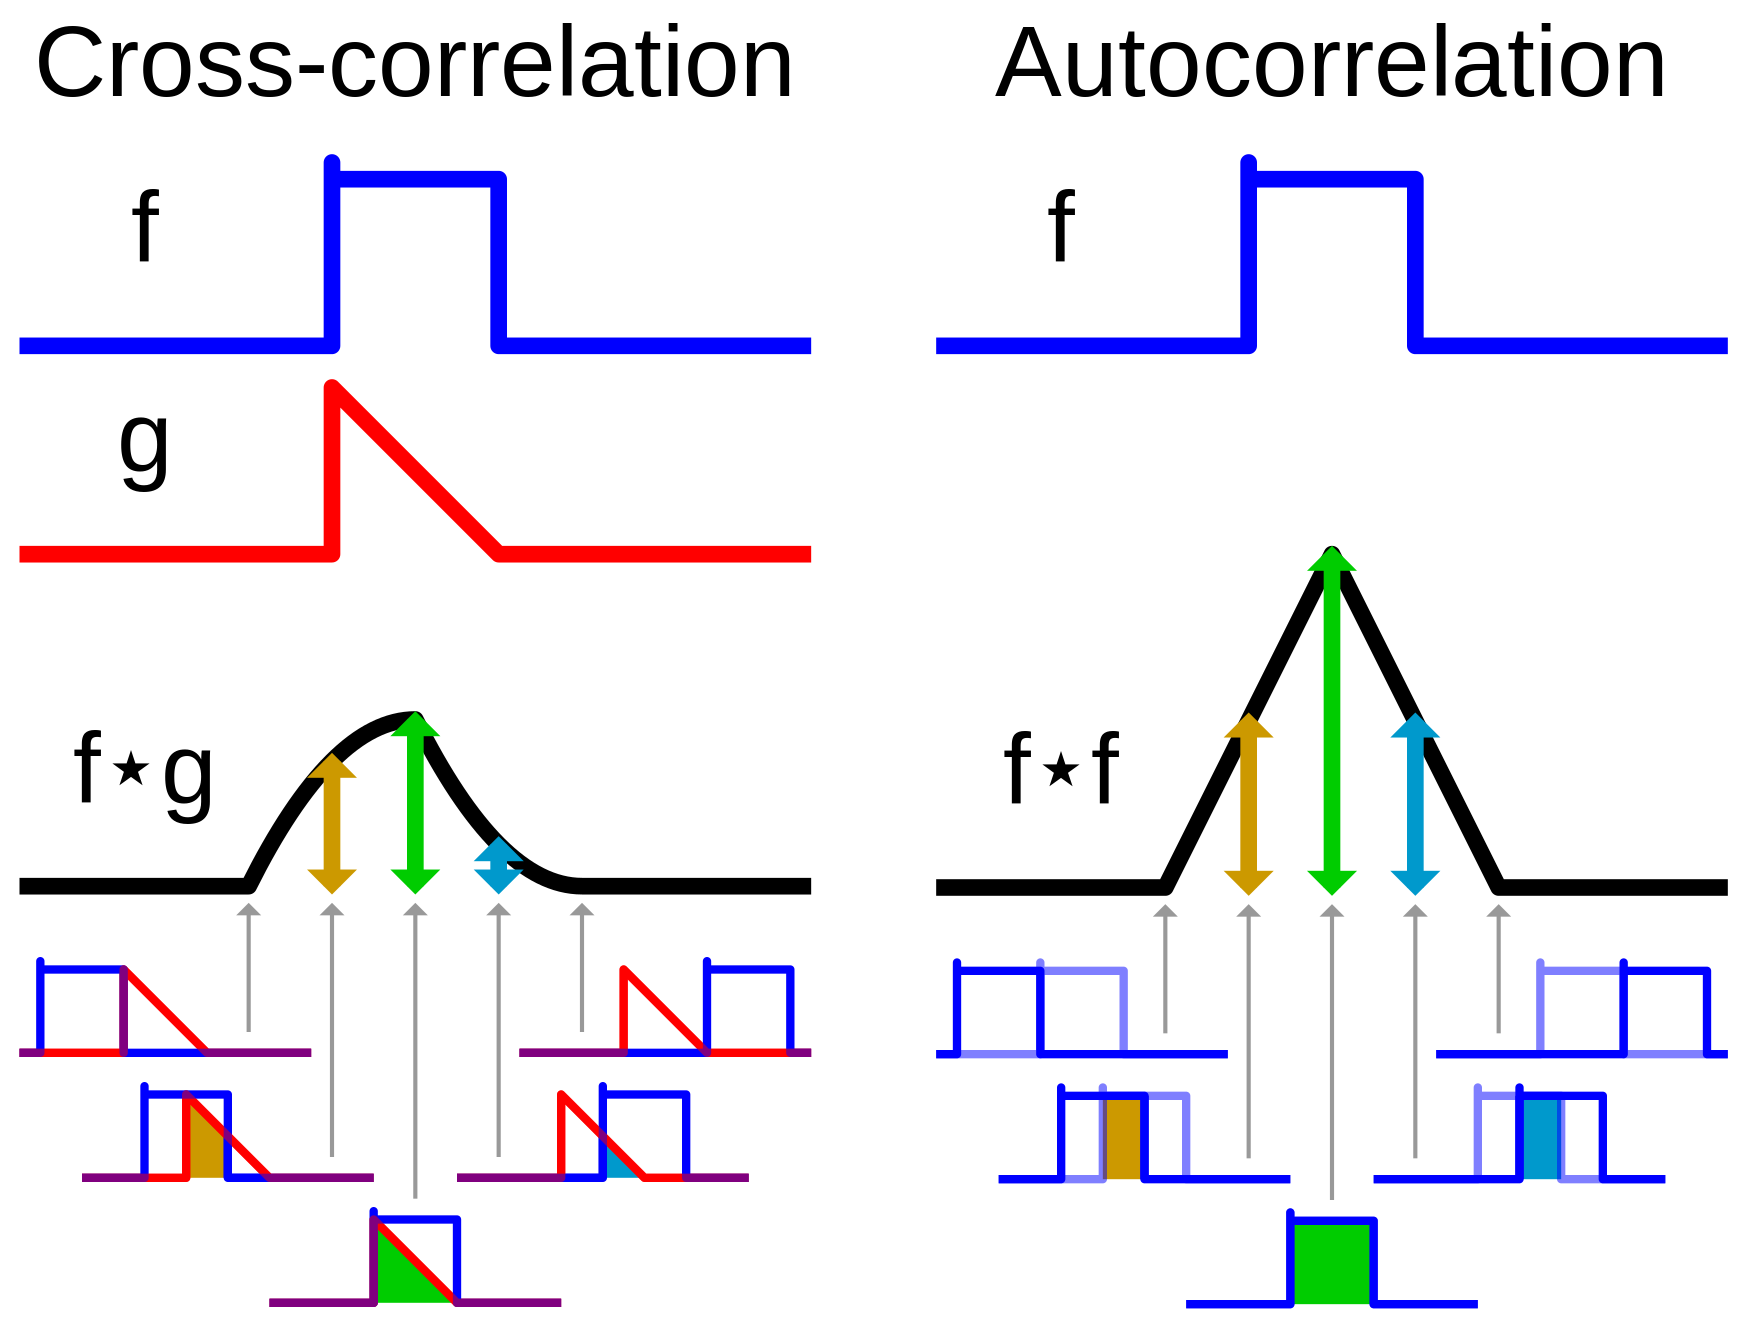
\includegraphics[height=0.8\textheight]{Comparison_convolution_correlation}
        \caption{Source: https://commons.wikimedia.org/wiki/File:Comparison\_convolution\_correlation.svg}
    \end{figure}
\end{frame}

\begin{frame}{Discrete Correlation}
\pnote{Rishi}
    \begin{figure}
        \centering
        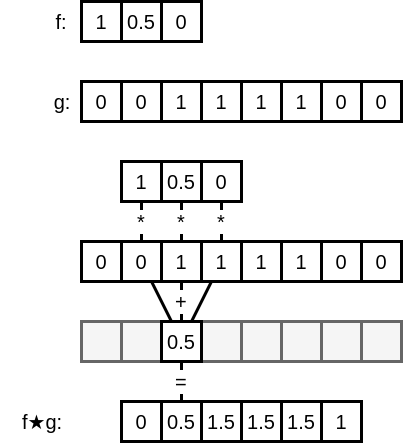
\includegraphics[height=0.7\textheight]{correlation.png}

    \end{figure}
\end{frame}

\begin{frame}{Discrete Autocorrelation}
\pnote{Rishi}
    \begin{figure}
        \centering
        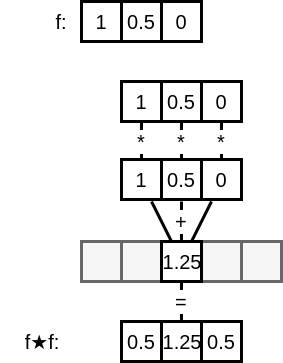
\includegraphics[height=0.7\textheight]{autocorrelation.png}

    \end{figure}
\end{frame}

\begin{frame}{Signal Transforms}
\pnote{Rishi}
\begin{itemize}
    \item Cosine Transform: Decompose signal into series of cosine functions with different frequencies
    \item Fourier Transform: Decompose signal into a series of complex exponentials (i.e., sines and cosines) representing different frequencies
    \item Cosine and Fourier transforms convert an input signal into its frequency domain; time information is essentially lost
    % TODO Show Wavelet scales
\end{itemize}
\end{frame}

\begin{frame}
\frametitle{Wavelets}
\pnote{Christina}
    \begin{itemize}
        \item Wavelet: A function that resembles a single oscillation of a wave
        \item Wavelets have both frequency and time domain info
        %\item Wavelets are not periodic
        % \item Wavelets can localize in time $\Longrightarrow$ efficient representation of discontinuities
        \item Wavelet functions are sharper; can represent discontinuities efficiently
    \end{itemize}
    
\begin{figure}
    \centering
    \begin{minipage}[b]{0.45\textwidth}
        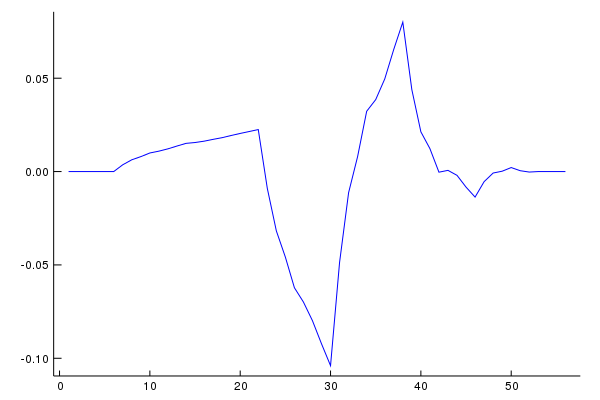
\includegraphics[width=\textwidth]{daub.png}
        \caption{Daubechies Wavelet}
    \end{minipage}
     \hfill
    \begin{minipage}[b]{0.45\textwidth}
        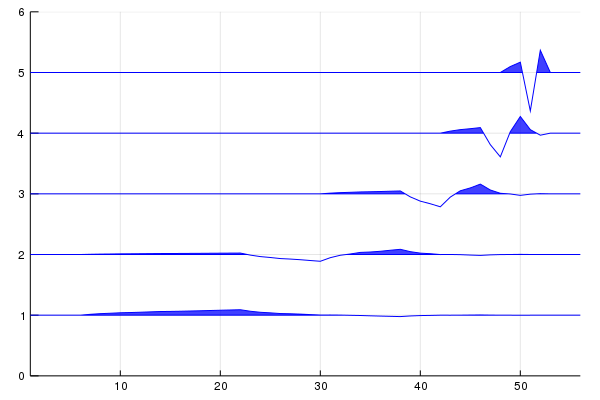
\includegraphics[width=\textwidth]{daub_wiggle.png}
        \caption{Daubechies Wavelets of various scales}
     \end{minipage}
\end{figure}
\end{frame}

\begin{frame}{Wavelet Transforms}
\pnote{Christina}
\begin{itemize}
    \item Represent a signal as a linear combination of wavelet basis functions
        \begin{align*}
            f(t) = \sum_{i=1}^n a_i \phi_i(t)
        \end{align*}
    where $a_i$ are expansion coefficients and $\phi(t)$ are the basis functions
    \item We use the \emph{redundant} version of the wavelet transform called \emph{maximal overlap discrete wavelet transform} (MODWT), which gives us \emph{shift-invariant} representation of an input signal.
\end{itemize}

\begin{figure} 
    \begin{minipage}[b]{0.45\textwidth}
        \centering
        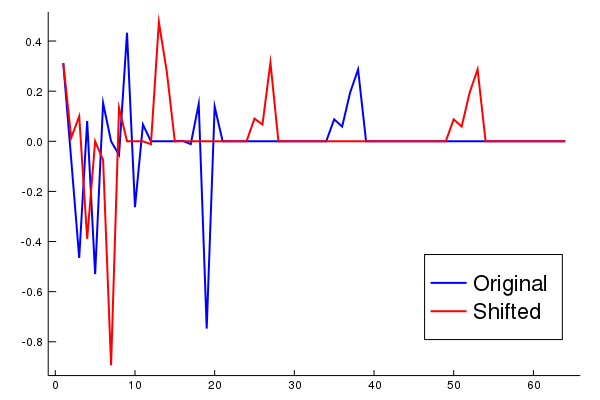
\includegraphics[width=0.85\textwidth,
            height=0.25\textheight]{shift_inv_dwt.png}
        \caption{Discrete Wavelet Transform Coefficients}
    \end{minipage}
     \hfill
    \begin{minipage}[b]{0.45\textwidth}
        \centering
        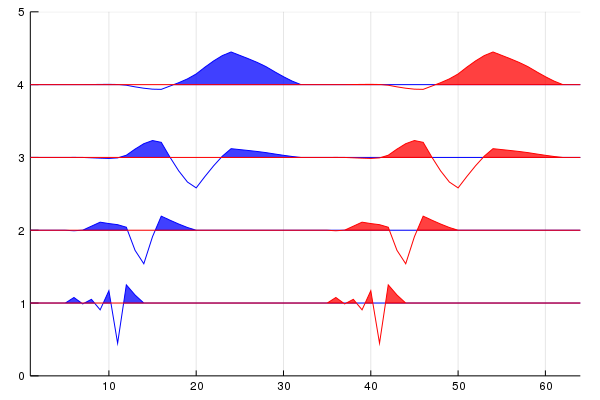
\includegraphics[width=0.85\textwidth,
            height=0.25\textheight]{shift_inv_modwt.png}
        \caption{MODWT Coefficients}
     \end{minipage}
\end{figure}
\end{frame}

\begin{frame}
\frametitle{Autocorrelation Functions of Wavelets}
\pnote{Christina}
    \begin{itemize}
        \item Autocorrelation properties: shift-invariant \textbf{and} symmetric
    \end{itemize}
    Original Signal
    \begin{figure}
        \centering
        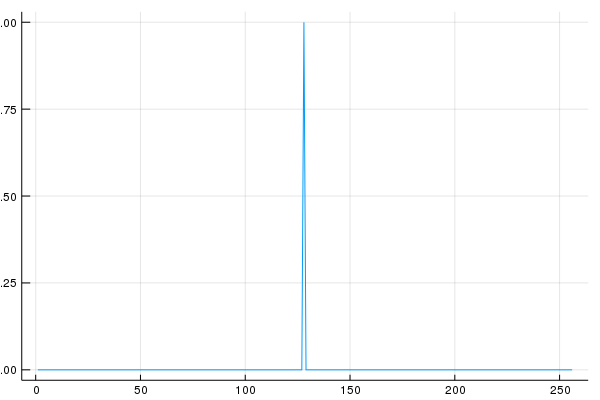
\includegraphics[height=0.1\textheight, width=0.7\textwidth]{spike_signal.png}
    \end{figure}

    \begin{columns}
        \column{.5\linewidth}
        \centering
            Autocorrelation WT
        \begin{figure}
            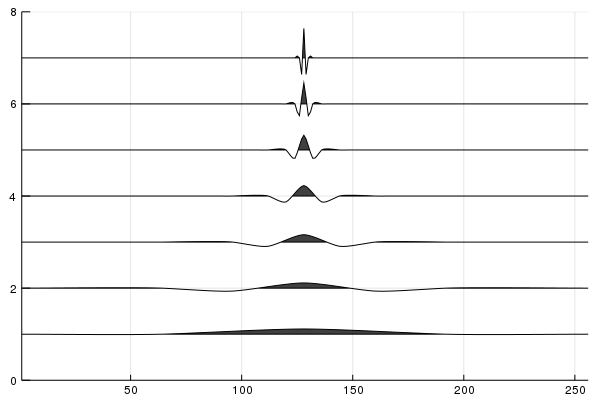
\includegraphics[width=\textwidth, height=0.5\textheight]{auto_decomposition.png}
        \end{figure}
        \column{.5\linewidth}
        \centering
            MODWT
            \begin{figure}
            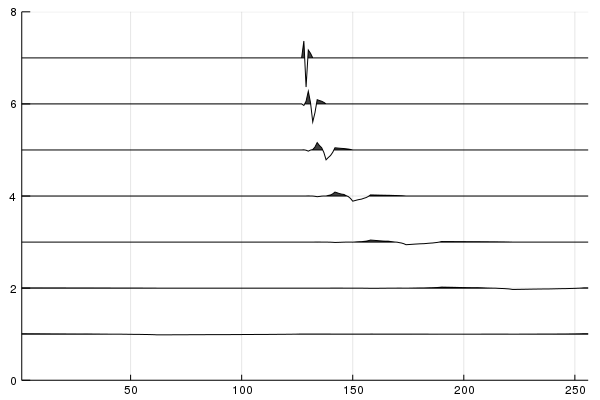
\includegraphics[width=\textwidth, height=0.5\textheight]{wavelet_decomposition.png}
            \end{figure}
    \end{columns}
    % \begin{figure}
    %     \centering
    %     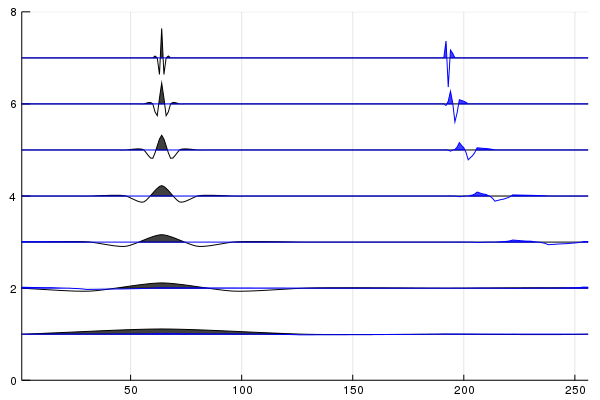
\includegraphics[height=0.4\textheight,width=7cm]{shift_inv.png}
    %     % TODO Show Time delayed MODWT
    % \end{figure}
\end{frame}

\begin{frame}
\frametitle{Data Analysis 1: Precipitation in the United States}
\pnote{Christina}
    \begin{figure}
        \centering
        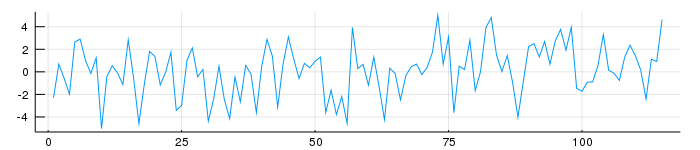
\includegraphics[height=0.17\textheight,width=0.78\textwidth]{precip.png}
        \setbeamerfont{caption}{size=\scriptsize}
        \caption{Original Signal}
        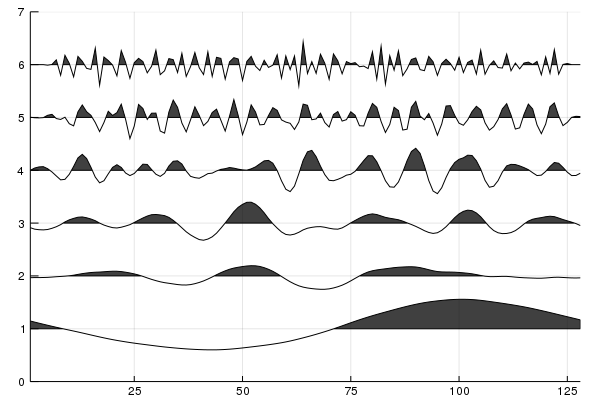
\includegraphics[height=0.45\textheight,width=0.75\textwidth]{precip_wiggle.png}
        \setbeamerfont{caption}{size=\scriptsize}
        \caption{Autocorrelation Wavelet Decomposition}
    \end{figure}
\end{frame}

\begin{frame}
\frametitle{Data Analysis 2: Stock Data}
\pnote{Rishi}
    \begin{figure}
        \centering
        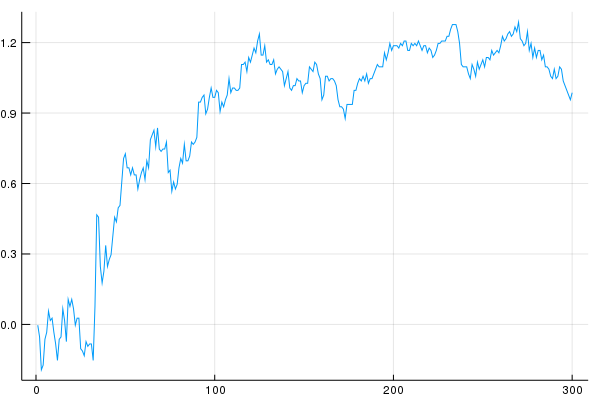
\includegraphics[height=0.17\textheight,width=0.78\textwidth]{stock_data_full.png}
        \caption{Original Signal}
        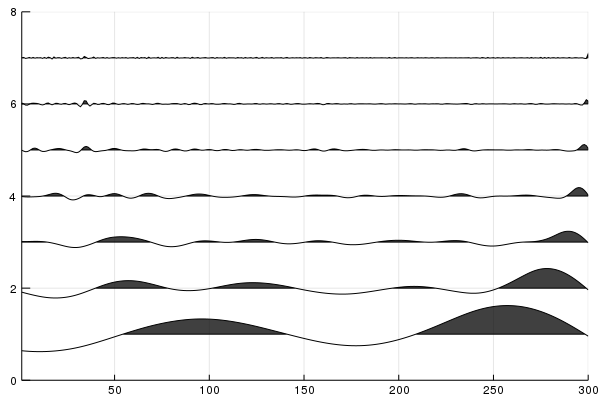
\includegraphics[height=0.3\textheight,width=0.75\textwidth]{stock_data.png}
        
        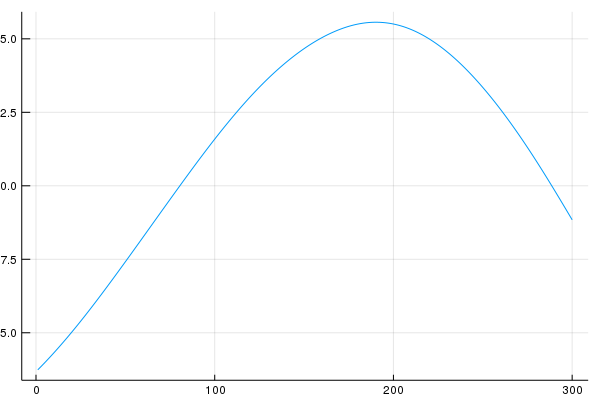
\includegraphics[height=0.15\textheight,width=0.75\textwidth]{stock_base.png}
        \caption{Autocorrelation Wavelet Decomposition}
    \end{figure}
\end{frame}

\begin{frame}
\frametitle{Data Analysis 3: Robot Movement}
\pnote{Rishi}
    \begin{figure}
        \centering
        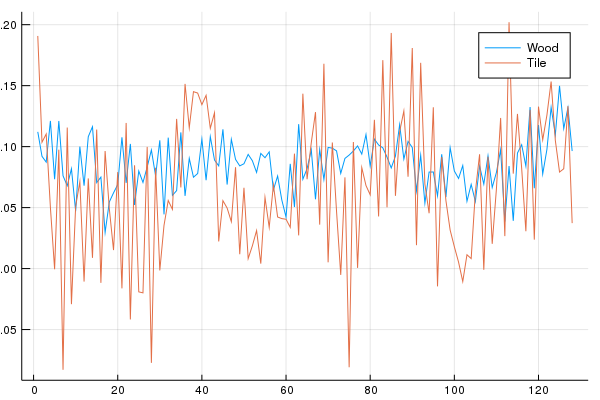
\includegraphics[height=0.17\textheight,width=0.78\textwidth]{wood_tile_plot.png}
        \caption{Original Signals}
        
        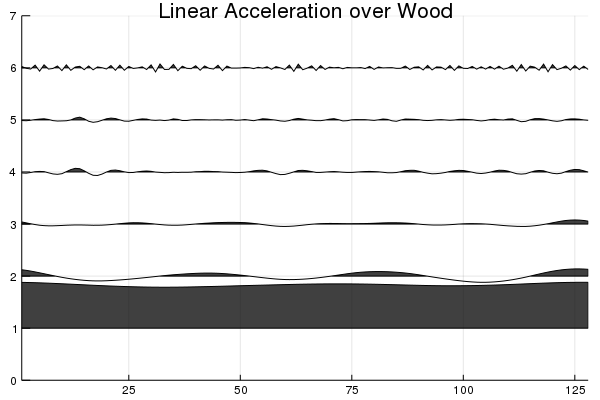
\includegraphics[width=0.5\textwidth]{wood_plot}
        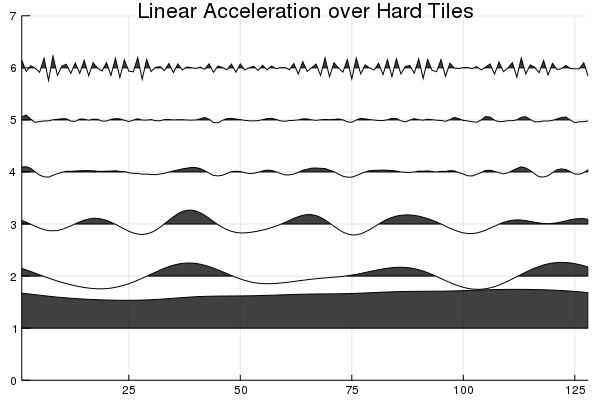
\includegraphics[width=0.5\textwidth]{tile_plot.png}
    \end{figure}
    
    
\end{frame}


\begin{frame}
\frametitle{Summary}
\pnote{Rishi}
\begin{itemize}
    \item Wavelets are functions that contain frequency and time information
    \item We can represent signals with a basis of wavelets
    \item The autocorrelation wavelet transform is superior to the maximum-overlap wavelet transform since it is both shift-invariant and symmetric
\end{itemize}
\end{frame}

\begin{frame}{}
  \centering \Huge
  Thank You
\end{frame}
\end{document} 